\documentclass[german,10pt,a4paper,twocolumn,colorscheme=darkblue]{orarticle}
\usepackage{epstopdf}
\usepackage{supertabular}

		
% ****************************************************************************** %
% ******************************** DOCUMENT ************************************ %
% ****************************************************************************** %
\begin{document}

%	\subject{Quick Manual}
	\title{Scarlet Gamma Manual}
	\authors{Johannes Jendersie, David Kuri, Florian Uhde}
	\abstract{Einführung}{
		Scarlet Gamma ist eine Pen \& Paper Plattform, die es ermöglicht in Echtzeit auf die Welt und die Spieleraktionen zu reagieren und alles zu verändern. Zum Beispiel ist es möglich Dungeons zu verändern, neue Räume und sogar neue Gegnertypen zu jedem Zeitpunkt einzuführen. Einige Aktionen wie das Kampfsystem sind auf das Pathfinder (D\&D) Regelwerk ausgelegt. Es ist aber auch möglich das Tool für andere Spielrunden einzusetzen. Dieses Dokument bietet eine Übersicht über die Funktionsweise und die wichtigsten Aktionen.
	}
	\maketitle

	\tableofcontents
	
	\section{Spieler und Spielleiter}
		Wie bei normalen P\&P-Runden übernimmt ein Spieler die Rolle des Spielleiters welcher absolute Macht hat. Dieser stellt auch den Server für das Spiel.
	
		\subsection{Neue Welten}
			Wählt man im Hauptmenü 'Spiel leiten' so wird der Server gestartet. In jedem Fall muss eine Welt geladen oder erstellt werden. Soll ein Abenteuer fortgesetzt werden muss der Name der existierenden Datei eingegeben werden. Andernfalls kann ein neuer Name gewählt und "Erstellen" gedrückt werden. Achtung: Dies überschreibt Welten, wenn die Datei bereits existierte.
			
			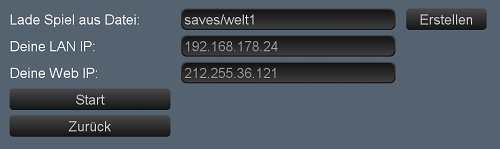
\includegraphics[width=\linewidth]{img/launch}
			
			Je nach dem ob Spieler sich im LAN oder über das Internet einloggen möchten sollten eine oder beide IP-Adressen notiert werden um sie den Spielern mitzuteilen, sobald die Welt geladen wurde.
			
		\subsection{Spielvorbereitung}
			Ähnlich der normalen Vorbereitung auf Papier sollte der Spielleiter die Welt für das Abenteuer planen und bauen. Dazu kann er nach dem Serverstart einfach neue Objekte und Karten erstellen wobei in dieser Zeit kein Spieler eingeloggt ist. Zusätzliche Vorbereitung auf Papier sind dabei möglich. Um Texte für NSCs zu schreiben empfiehlt es sich dies in Extra-Textdateien zu speichern und später an den entsprechenden Stellen in den Chat einzufügen.
		
		\subsection{Einem Spiel beitreten}
			Nach wählen der Option 'Spiel beitreten' im Hauptmenü muss eine Verbindung zum gestarteten Server hergestellt werden. Welche IP-Adresse dieser hat wird beim Starten des Servers angezeigt.
			
			Es kann passieren, dass eine Firewall die Verbindung verhindert. Dann muss eine entsprechende Regel für Scarlet Gamma hinzugefügt werden. Im Spiel über das Internet ist außerdem darauf zu achten, dass der Port 42961 freigegeben ist.
			
			Anschließend wird die Welt übertragen und eine Liste mit existierenden Spielern darin angezeigt. Wird eine Abenteuer fortgesetzt reicht ein Klick. In einer neuen Welt oder wenn ein neuer Charakter hinzukommt kann dieser über 'Neuer Spieler' erstellt werden.
		
	\section{Komponentenbasiertes Objektsystem}
		Alles in der Welt folgt dem gleichen Schema um ein größtmögliche Kombinationsvielfalt zu ermöglichen. Jedes Objekt kann eine beliebige Anzahl an Eigenschaften enthalten. Eine Eigenschaft besteht aus einem Namen, einem Wert und kann Objekte enthalten.
		
		Ein Wert kann im Prinzip beliebig gesetzt werden. In einigen Fällen erwartet das System allerdings Zahlen oder Formeln. Beispiel $('IN'-10)/2$: $'IN'$ referenziert dabei die gleichnamige Eigenschaft im selben Objekt, welche zuerst ausgewertet wird. Die Division rundet immer ab. Endlosschleifen werden nicht detektiert.
		
		Die folgende GUI wird verwendet um Objekte und Eigenschaften zu bearbeiten.
		
		\begin{minipage}{0.5\linewidth}
		\begin{picture}(0,130)
			\put(0,0){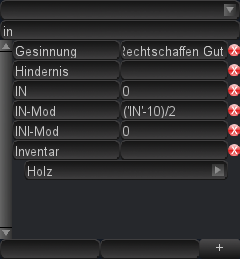
\includegraphics[width=\linewidth]{img/propertygui}}
			\put(10,120){\colorbox[rgb]{1.0, 1.0, 0.9}{\tiny 1}}
			\put(55,42){\colorbox[rgb]{1.0, 1.0, 0.9}{\tiny 1}}
			\put(55,75){\colorbox[rgb]{1.0, 1.0, 0.9}{\tiny 2}}
			\put(110,75){\colorbox[rgb]{1.0, 1.0, 0.9}{\tiny 3}}
			\put(55,110){\colorbox[rgb]{1.0, 1.0, 0.9}{\tiny 4}}
			\put(55,5){\colorbox[rgb]{1.0, 1.0, 0.9}{\tiny 5}}
		\end{picture}
		\end{minipage}
		\begin{minipage}{0.49\linewidth}
		\footnotesize
		\begin{description}
			\item[1] Name des Objekts sofern die Eigenschaft existiert.
			\item[2] Eig.: Name + Wert
			\item[3] Eig. aus Objekt löschen.
			\item[4] Filter: Alle Eig., die Eingabe enthalten werden gezeigt.
			\item[5] Neue Eig. hinzufügen. Der Wert kann später noch geändert werden, der Name nur durch Löschen und Neueinfügen.
		\end{description}
		\end{minipage}
		
		Generell gilt, das nicht jeder alles darf. Je nach Rechten sind einige der Optionen nicht verfügbar.
	
		\subsection{Besondere Eigenschaften}
			Manche der Eigenschaften erlauben besondere Tätigkeiten auf dem Objekt, wenn es im Spiel platziert ist. Diese sind in Modulen zusammengefasst um Objekte schneller bauen zu können.\\
			
			\begin{supertabular}{p{0.275\linewidth}|p{0.62\linewidth}}
				\textbf{Angreifbar} [Modul]      & Ein Objekt das 'TP' (Trefferpunkte) und 'RK' (Rüstungsklasse) enthält kann angegriffen werden. \\\hline
				\textbf{Besitzer} [Eigenschaft]  & Wenn diese Eigenschaft nicht leer ist kann ein Spieler das Objekt beobachten. Wenn der Spielername gleich dem Wert ist kann der Spieler das Objekt steuern.\\\hline
				\textbf{Farbe} [Eigenschaft]     & Multipliziert die Textur des Objekts mit der Farbe. Hexadezimal: rrggbbaa. Beispiel: 008800ff = mittleres grün.\\\hline
				\textbf{Hindernis} [Eigenschaft  & Felder mit mindestens einem Hindernis können nicht betreten werden.\\\hline
				\textbf{Schalter} [Modul]        & Kann umgeschaltet werden, was eine Meldung beim Spielleiter zur folge hat. Der Wert ist 'true' oder 'false'\\\hline
				\textbf{Sprungmarke} [Modul]     & Spielleiter kann ein Objekt als Sprungziel wählen (auch auf einer anderen Karte). Später können Spieler diese als Teleport/Treppe/... verwenden.\cr
			\end{supertabular}
			
	\section{Editor}
		\begin{picture}(0,120)
			\put(0,0){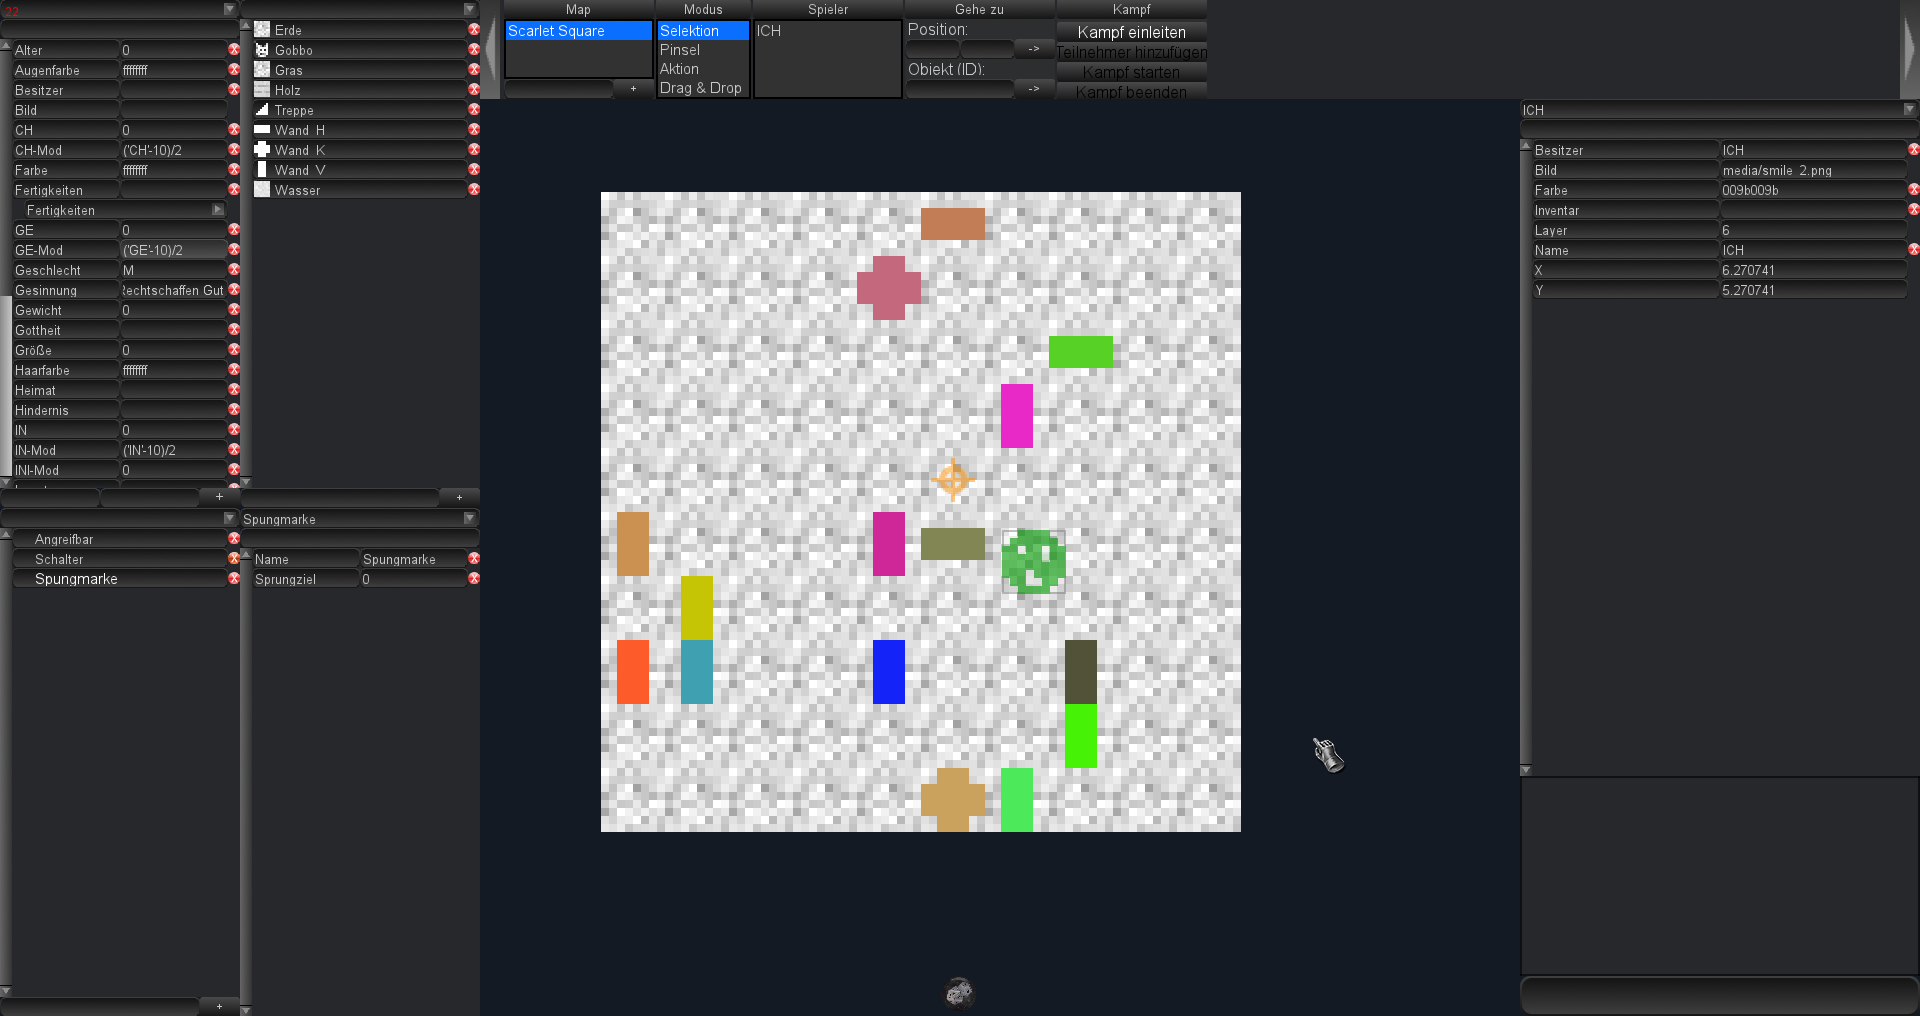
\includegraphics[width=\linewidth]{img/master}}
			\put(10,90){\colorbox[rgb]{1.0, 1.0, 0.9}{\tiny 1}}
			\put(10,42){\colorbox[rgb]{1.0, 1.0, 0.9}{\tiny 2}}
			\put(40,90){\colorbox[rgb]{1.0, 1.0, 0.9}{\tiny 3}}
			\put(40,42){\colorbox[rgb]{1.0, 1.0, 0.9}{\tiny 4}}
			\put(80,115){\colorbox[rgb]{1.0, 1.0, 0.9}{\tiny 5}}
			\put(207,90){\colorbox[rgb]{1.0, 1.0, 0.9}{\tiny 6}}
			\put(207,10){\colorbox[rgb]{1.0, 1.0, 0.9}{\tiny 7}}
		\end{picture}
		
		\begin{description}
			\item[1] Liste aller verfügbaren Eigenschaften. Der Spielleiter kann sich auch beliebige weitere Eigenschaften ausdenken. Eigenschaften können per Drag\&Drop nach \textbf{4} und \textbf{6} kopiert werden.
			\item[2] Liste der Module. Ein klick zeigt alle Eigenschaften des Moduls in \textbf{4}. Module können editiert und weitere hinzugefügt werden um Eigenschaften zu gruppieren. Module können per Drag\&Drop nach \textbf{4} und \textbf{6} kopiert werden.
			\item[3] Liste der Objekt-Templates. Diese sollte die Menge aller möglichen Objekte in der Welt beinhalten. Ein Objekt (Kopie) kann per Drag\&Drop in der Welt oder in einer Property platziert werden. Außerdem kann das selektierte Objekt mit dem Pinsel hinzugefügt werden. Das Selektieren zeigt den Inhalt in \textbf{4} an.
			\item[4] Anzeige für selektiertes Modul oder Template.
			\item[5] Toolbar
			\item[6] Anzeige für selektierte Objekte auf der Karte. Es werden immer nur die Eigenschaften gezeigt, die in allen Objekten enthalten sind. Aktionen und Änderungen beziehen sich immer auf alle Objekte. Die Eigenschaften können Editiert werden oder per Drag\&Drop von \textbf{1, 2, 3} und der Map befüllt / erweitert werden.
			\item[7] Der Chat inklusive Statusmeldungen
		\end{description}
		
		\subsection{Toolbar}
		\subsubsection*{Map}
			Eine Liste mit allen Karten der geladenen Welt. Es kann per Klick zwischen den Karten gesprungen werden und neue Karten erstellt werden.
		\subsubsection*{Modus}
			Verschiedene Spielsituationen können unterschiedliche Anforderungen stellen. Die Modi unterscheiden möglichst sinnvolle Aktionen der Maus. Der Rechtsklick ist immer gleich belegt siehe Aktionen \ref{Aktionen}.
			
			\textbf{Selektion}: Linksklick selektiert oberstes sichtbares Objekt. Links+ziehen eines Rechtecks markiert alle sichtbaren Objekte.
			
			\textbf{Pinsel}: Blendet das Pinsel-tool ein. Linksklicks/Moves verändern entsprechend die Map.
			
			\textbf{Aktion}: Linksklick lässt alle markierten Objekte eine Standardaktion ausführen. Neuselektion kann nach wie vor durch den Rechtsklick vorgenommen werden.
			
			\textbf{Drag \& Drop}: Objekte können auf der Karte verschoben werden.
						
		\subsubsection*{Pinsel}
			\begin{minipage}{0.49\linewidth}
			\textbf{Ersetzen} wird alle Objekte des Ziel-Layers löschen und das Objekt aus der Template-Liste einfügen.
			
			\textbf{Hinzufügen} Wird ausschließlich Objekt erzeugen und keine löschen.
			
			\end{minipage}\hspace{1em}
			\begin{minipage}{0.45\linewidth}
				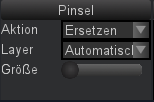
\includegraphics[width=1.0\linewidth]{img/brush}
			\end{minipage}
			
			\textbf{Löschen} Löscht Objekte mit gleichem Namen, wie das gewählte Objekt.

			\textbf{Layer} Es gibt 10 Schichten, in die Objekte eingefügt werden. Diese sind vor allem für die Anzeige wichtig. Automatisch wird im Objekt nach einer Layer-Eigenschaft suchen. Kann diese nicht gefunden werden wird das Objekt in Schicht 10 (Eigenes II) eingefügt.
			
			\textbf{Größe} Größe des Pinsels. Dieser ist quadratisch, da sich so besser Gebäude bauen lassen.
		
		\subsubsection*{Spieler}
			Enthält eine Liste mit allen Spielern. Ein Klick selektiert den Spieler und setzt die Ansicht auf den Spieler. Der Spieler kann per Drag\&Drop auf die Karte gesetzt bzw. versetzt werden.
		\subsubsection*{Gehe zu}
			Tool zur Erleichterung der Navigation. Es kann entweder zu einer Tile-Position oder zu einem Objekt gesprungen werden. Für zweiteres benötigt man die Objekt-ID, welche zb. in der Sprungziel Eigenschaft steht.
		\subsubsection*{Kampf}
			Kampf mit aktueller Auswahl einleiten, danach nach belieben weitere Teilnehmer hinzufügen oder Kampf beginnen. Teilnehmer machen Initiativewürfe und erscheinen dann in der Liste unten links. Nur der aktive Teilnehmer kann handeln.
		
	\section{Chat}
		In der Chat-Zeile können neue Nachrichten für alle angegeben werden. Eine Möglichkeit Spieler direkt anzuschreiben existiert derzeit nicht.
		
		Die Nachrichtenzeile kann mit 'Enter' oder einem Klick fokussiert werden. Hat das Feld den Fokus sendet 'Enter' die Nachricht.
		
		Folgende besondere Eingaben sind möglich:
		\begin{description}
		\item[/me TEXT] Schreibt deinen Namen mit dem Text in Emotefarbe. '\textit{/me isst einen Keks}' $\rightarrow$ '\textit{Johannes isst einen Keks}'
		\item[/e TEXT] Schreibt den TEXT in Emotefarbe. '\textit{/e Das Wetter verschlechtert sich}' $\rightarrow$ '\textit{Das Wetter verschlechtert sich}' (wer hätte es geahnt)
		 \item[/npc NAME TEXT] Lässt den NSC etwas sagen. '\textit{/npc Hans Du bist mir eine Wurst}' $\rightarrow$ '\textit{[Hans] Du bist mir eine Wurst.}
		\end{description}
	
	\section{Der Spielfluss}
		\subsection{Aktionen}
			\label{Aktionen}
			Aktionen werden immer für alle selektierten Objekte (entspricht ausführenden) durchgeführt. Die Aktion bezieht sich immer auf ein Ziel, das wie folgt gewählt werden kann:
			
			\begin{minipage}{0.54\linewidth}
			Ein Rechtsklick öffnet ein Kreismenü mit allen Objekten des Feldes. Ein Rechtsklick auf das Objekt (einen der Buttons) zeigt Aktionsmöglichkeiten. Der Spieler kann die Aktionen auch mit einem Linksklick anzeigen lassen, im Falle des Spielleiters selektiert der Linksklick das Objekt.
			\end{minipage}\hspace{1em}
			\begin{minipage}{0.4\linewidth}
				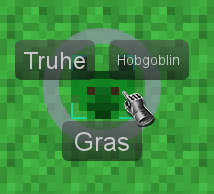
\includegraphics[width=1.0\linewidth]{img/circularmenu}
			\end{minipage}
			
			Spieler und Spielleiter (im Aktionsmodus) können mit einem Linksklick direkt auf das Feld eine vorgegebene Aktion ausführen. Diese wird aus allen Aktionen auf allen Objekten des Feldes ausgewählt. Es passiert nichts, wenn es keine gültige Option gibt.
		
			Der Spieler kann durch alle anderen Spieler/Tiergefährten (alles mit Besitzer-Eigenschaft) scrollen und wenn sie ihm gehören auch steuern.
			
		\subsection{Pause}
			Der Spielleiter kann die Simulation sich bewegender Objekte anhalten und dabei alle Spieler sperren, sofern er in ruhe etwas editieren möchte.
		
		\subsection{Kämpfe}
			\subsubsection*{Start und Initiative}
			Über die Toolbar kann der Spielleiter einen Kampf einleiten. Alle ausgewählten Objekte werden direkt zum Kampf hinzugefügt, weitere Objekte können über die entsprechende Schaltfläche später hinzugefügt werden. Von jedem Objekt wird ein Initiativewurf verlangt, der die Kampfreihenfolge festlegt. Diese Reihenfolge wird Spielern und Spielleiter unten Links angezeigt, solange der Kampf andauert. Ist die Initiativereihenfolge von allen Teilnehmern eingegangen kann der Kampf über die Schaltfläche `Kampf starten' begonnen werden.
			\subsubsection*{Runden}
			Der Teilnehmer mit der höchsten Initiative beginnt. Jede Runde besteht aus einer Standard- sowie einer Bewegungsaktion. Die Standardaktion besteht in der Regel aus einem Angriff, kann jedoch z.B. durch das Untersuchen eines Objektes ersetzt werden. Die Bewegunsaktion erlaubt Bewegung bis zur Bewegungsrate des Objektes oder das Ausführen einer bewegungsentsprechenden Aktion. Hat sich ein Teilnehmer in seiner Runde nicht bewegt (aber möglicherweise eine bewegungsentsprechende Aktion benutzt) steht ihm ein 1,5m-Schritt zur Verfügung. Nach der Runde muss jeder Teilnehmer, ob vom Spieler oder Spielleiter kontrolliert, seine Runde beenden. Die entsprechende Schaltfläche findet sich unten links.
			
	\section{Shortcuts}
		Im folgenden ist die Tastaturbelegung aufgelistet. [M] bedeutet, dass die Aktion im Master-Modus, also dem Spielleiter zur Verfügung steht. [S] bedeutet entsprechend, dass der Spieler die Aktion ausführen kann.\\
		
		\begin{supertabular}{p{0.15\linewidth}|p{0.075\linewidth}|p{0.62\linewidth}}
%								     & Wer & Keyboard\\\hline
			\textbf{C}               & M,S & Öffnet den Charakterbildschirm für das ausgewählte Objekt (M) oder den Spieler. \\\hline
			\textbf{Alt+1 ... Alt+0} & M & Ändere Sichtbarkeit der Layer 1 bis 10. \\\hline
			\textbf{Alt}             & M & Blende alle Layer wieder ein.\\
			                         & S & Setze Fokus auf den Spieler.\\\hline
			\textbf{Entf}			 & M & Lösche alle selektierten Objekte.\\\hline
			\textbf{Esc}			 & M,S & In den meisten Menüs: zurück.\\\hline
			\textbf{Pause, P}		 & M & Halte Spiel an oder setze fort.\\\hline
			\textbf{Strg+1 ... Strg+9}& S,M & Setze Shortkey für ein selektiertes Objekt*.\\\hline
			\textbf{1 ... 9}		 & M,S & Gehe zu Objekt auf Hotkey 1-9.\\\hline
			\textbf{Strg+C}			 & M,S & Kopieren von markiertem Text.\\\hline
			\textbf{Strg+V}			 & M,S & Einfügen von markiertem Text.\\\hline
			\textbf{Strg+ Selektieren}& M & Objekte der Auswahl hinzufügen.\\\hline
			\textbf{Tab, Shift+ Tab}	 & S & Durch alle beobachtbaren Objekte schalten.\cr
		\end{supertabular}\\
	
		* Für den Spieler ist das immer das fokussierte Objekt, welches er durch Tab/Shift+Tab erreichen kann. Der Master kann die Keys derzeit auch nur für einzelne Objekte definieren (Gehe zu wäre bei mehreren undefiniert).
	
\end{document}